\documentclass[sigconf, nonacm]{acmart}
% PVLDB Vol. 20 template: acmart.cls v2.19 + pvldb.sty, pinned copies from github.com/vldbproceedings/VLDB-Template.
% The whole paper is in this one file. Generated regions (% >>> ... % <<<) are replaced in place by make and the table script.
%%% VLDB block start %%%
\usepackage{pvldb}
%%% VLDB block end %%%
\renewcommand\vldbdoi{XX.XX/XXX.XX}
\renewcommand\vldbpages{XXX-XXX}
\renewcommand\vldbavailabilityurl{https://github.com/Xyc-arch/specbridge-artifact}
\setkeys{acmart.cls}{balance=false}
\usepackage{booktabs}
\usepackage{tabularx}
\usepackage{array}
\usepackage{amsmath}
\usepackage{placeins}

\usepackage{algorithm}
\usepackage{algpseudocode}
\setlength{\emergencystretch}{1em}
\setcounter{dbltopnumber}{3}
\hypersetup{hidelinks}
\AtBeginDocument{\color{black}}
\newcommand{\system}{SpecBridge}
% the supplement's labels (its \newlabel lines, prefixed ext-): make writes them here from supplement.aux, so the paper
% compiles alone, e.g. on Overleaf
% >>> labels supplement (written by make from supplement.aux; do not edit by hand)
\AtBeginDocument{%
\newlabel{ext-sec:datamap}{{A}{1}{Data and Experiments}{appendix.A}{}}
\newlabel{ext-sec:appendixlibrary}{{B}{1}{The Choices Are Common}{appendix.B}{}}
\newlabel{ext-sec:catalogue}{{B}{1}{The Choices Are Common}{appendix.B}{}}
\newlabel{ext-tab:librarydetail}{{S1}{1}{All choice types (Figure~\ref {fig:choices} of the paper shows the major ones). Library: choices of meaning in benchmark failures, open (the wording fits both interpretations) or settled (it selects one). References: BIRD and Spider questions silent on the choice, by the interpretation their reference SQL takes: the usual one, or the other with its share (\%), after the less common interpretations were reviewed; --: not readable from the SQL. Sets: the 204 accepted request sets, of the types whose other interpretation at least 1\% of silent references take. The library's value-representation type is split by its SQL edit: comparison strictness is a strict cutoff, any other edit value matching.\relax }{table.caption.3}{}}
\newlabel{ext-fig:datamap}{{S1}{2}{Data and experiments: sources (top), data built from them (middle), and the experiments with their sample sizes (bottom). Arrows show what is built from what and what each experiment uses.\relax }{figure.caption.1}{}}
\newlabel{ext-sec:cases}{{C}{2}{Calculation Choices with Real Consequences}{appendix.C}{}}
\newlabel{ext-tab:catbreadth}{{S2}{3}{Top: every library choice (Table~\ref {tab:librarydetail}), by the benchmark whose failures revealed it. Bottom: every accepted request set, by the source of its database. DBs: distinct databases.\relax }{table.caption.8}{}}
\newlabel{ext-sec:filtersets}{{D}{3}{Request Sets with Filter Conditions}{appendix.D}{}}
\newlabel{ext-sec:querydetails}{{E}{3}{Query Generation Details}{appendix.E}{}}
\newlabel{ext-eq:reach}{{2}{3}{Query Generation Details}{equation.E.2}{}}
\newlabel{ext-sec:furtherdetails}{{F}{3}{Seeds, Versions and Selection Rules}{appendix.F}{}}
\newlabel{ext-tab:cases}{{S3}{4}{Documented cases where one calculation choice changed a consequential number or decision, by domain, with the closest choice type in our library.\relax }{table.caption.10}{}}
\newlabel{ext-tab:filtersets}{{S4}{4}{Filter request sets (43 accepted), per model: both specific requests right (with exploration); among those, open requests answered with both interpretations; open requests that name the choice (Opus judge); specific requests right (single call); missed interpretations the model computes when asked, of all missed.\relax }{table.caption.12}{}}
\newlabel{ext-tab:construction}{{S5}{4}{Program construction on 12 databases, with no model calls after catalogue preparation. Every delivered SQL is distinct, has the requested depth, and passes both integrity checks.\relax }{table.caption.17}{}}
\newlabel{ext-alg:families}{{S1}{4}{Build a request set around one calculation choice\relax }{algorithm.1}{}}
\newlabel{ext-fig:ablation}{{S2}{5}{Generation outcomes with each construction rule removed (2,350 attempts). The labels give the share valid, on target and sound.\relax }{figure.caption.14}{}}
\newlabel{ext-fig:specification}{{S3}{5}{Exact description versus natural request on 382 generated tasks. Left: accuracy; numbers give the difference in points. Right: errors from the exact description by step depth.\relax }{figure.caption.15}{}}
\newlabel{ext-fig:coverage}{{S4}{5}{Features the generator can build, as a share of 152 databases: possible by the schema, and generated and accepted.\relax }{figure.caption.16}{}}
\newlabel{ext-sec:typeexamples}{{G}{5}{Examples of Each Choice Type}{appendix.G}{}}
\newlabel{ext-tab:catlibrary}{{S6}{6}{Examples of Each Choice Type}{table.6}{}}
\newlabel{ext-tab:catsets}{{S7}{7}{Examples of Each Choice Type}{table.7}{}}
}
% <<< labels supplement
\newcommand{\ext}[1]{Appendix~\ref{ext-#1} of the supplement}\newcommand{\extref}[1]{\ref{ext-#1}}
\newcommand{\spec}{\ensuremath{V}}
\newcommand{\sql}[1]{\textnormal{\texttt{#1}}}
\newcolumntype{Y}{>{\raggedright\arraybackslash}X}
\graphicspath{{figures/}}
\title{Text-to-SQL Models Make Choices Without Saying So [Experiment, Analysis \& Benchmark]}
\author{Yichen Xu}
\affiliation{%
  \institution{University of California, Berkeley}
  \city{Berkeley}
  \state{CA}
  \country{USA}
}
\email{yichen\_xu@berkeley.edu}
\author{Shipei Lin}
\affiliation{%
  \department{School of Data Science}
  \institution{The Chinese University of Hong Kong, Shenzhen}
  \city{Shenzhen}
  \country{China}
}
\email{225045017@link.cuhk.edu.cn}
\author{Chenhao Ma}
\affiliation{%
  \department{School of Data Science}
  \institution{The Chinese University of Hong Kong, Shenzhen}
  \city{Shenzhen}
  \country{China}
}
\email{machenhao@cuhk.edu.cn}
% Float spacing with little stretch, so a column is not filled by blank space below a figure.
\setlength{\textfloatsep}{12pt plus 2pt minus 2pt}\setlength{\floatsep}{10pt plus 2pt minus 2pt}\setlength{\dbltextfloatsep}{12pt plus 2pt minus 2pt}\setlength{\dblfloatsep}{10pt plus 2pt minus 2pt}
\begin{document}
\begin{abstract}
A text-to-SQL answer can run, return a plausible number and still compute something other than what the analyst meant. This happens when a request leaves a calculation choice open, such as whether to count rows or entities, and the model settles the choice without saying so. Benchmarks cannot detect this, because they score one reference interpretation even where the question leaves the choice open. This paper introduces \system{}, a framework that tests what a model does with such a choice by changing only that choice. A request set holds three requests on the same data, one for each of two interpretations and one that leaves the choice open, and execution scores every answer. \system{} builds request sets on real databases from choices mined from benchmark failures. On 204 hand-validated request sets, four models usually compute both interpretations when each is asked for, yet for the open request they return both interpretations in only 15--58\% of those sets, and they name the choice in only 38--70\% of all sets. When they settle a choice silently, they take the interpretation that benchmark references take by convention, and on BIRD over two in five of the answers scored wrong on such questions return the other interpretation. A method that first decides whether a request leaves a choice open and then answers each interpretation in its own call returns every interpretation for 29 to 63 points more open requests than the single answer that production assistants return, with no loss of precision, and is more precise than plain prompting, sampling and disambiguate-then-parse, at 2.6 calls per request, and needs fewer user turns than asking the user. After the user picks, adding the pick as one clause beats rewriting the request with DtP's or LangChain's prompts by 8.5 to 10.5 points.
\end{abstract}
\keywords{text-to-SQL, database interfaces, evaluation, controlled tests, ambiguity, language models}
\maketitle
%%% VLDB block start %%%
\vldbtopmatter
%%% VLDB block end %%%
% ===== introduction =====
\section{Introduction}
\label{sec:intro}
Analysts increasingly ask for numbers in natural language and get them from a text-to-SQL system, often without reading the SQL. For these users a query that fails is safe, because the error is visible. The dangerous answer is a query that runs and returns a plausible number, computed differently than the analyst meant. Outside SQL, such small calculation choices have had large consequences. A finding that high public debt slows growth depended on averaging within each country before averaging across countries~\cite{herndon2014debt}, and a health-care algorithm that measured need by cost cut the Black patients chosen for extra care by more than half~\cite{obermeyer2019bias}. A text-to-SQL system makes such choices on every request, and its user sees only the result. We call such a choice, settled without telling the user, a silent choice. The answer is correct for one interpretation, so checks that look for wrong SQL~\cite{chen2023error,alrashed2026verification} do not catch it.

Take ``the average rental price per day'' for each film rating (Figure~\ref{fig:teaser}). It can be computed two ways, which we call interpretations. Interpretation A averages each film's daily price, and interpretation B divides the average price by the average rental length. For two films priced at \$6 for two days and \$6 for six days, the first interpretation gives \$2.00 per day and the second \$1.50. Both are simple SQL, and on the \texttt{sakila\_1} database the two interpretations differ for every rating. For the request as worded, which leaves this choice open, all four models we test, Claude Haiku~4.5, Claude Sonnet~5.5, GPT-6 Sol and GPT-6 Luna (Haiku, Sonnet, GPT-Sol and GPT-Luna below), return A. Sonnet and GPT-Luna say that there is a choice, but only Sonnet also gives B, the ratio of two averages.

% Built from figures/src/diag_teaser.tex with pdfLaTeX (the paper's fonts); included at 1:1. Make in paper/tex rebuilds it.
% Teaser values are real: sakila_1 film table (A = AVG(rental_rate / rental_duration), B = AVG(rental_rate) / AVG(rental_duration),
% per rating). Model outcomes are the recorded single-call responses to the open film request
% (out/transfer/eval12-v2/render/disclose/*/...06768b2b94__open.json).
\begin{figure}[t]
\centering
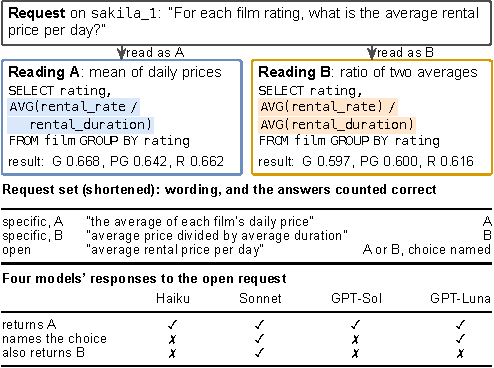
\includegraphics{diag_teaser.pdf}
\caption{One request, two correct interpretations (shaded: the SQL that differs), and four models' responses. Each specific request asks for one interpretation; the open request keeps the user's original wording unchanged.}
\Description{A request on the film table leads to two interpretations, A (mean of daily prices) and B (ratio of means): the SQL expression
that differs, and their different per-rating values. Below, the three requests of the request set, and a table of four models' recorded responses to the open request.}
\label{fig:teaser}
\end{figure}

A reliable text-to-SQL system must compute the interpretation that a specific request asks for, report a choice that a request leaves open together with the other interpretation, and stay quiet about a choice that the wording already settles. Benchmarks such as Spider and BIRD measure only the first. They score each question against one reference interpretation, even where the question leaves the choice open, so a model that guesses the authors' interpretation scores as well as one that reports the choice. On 79 BIRD questions whose answer the choice changes, accepting both interpretations raises accuracy from 25\% to 57\% (Section~\ref{sec:impact}), so part of the gap between the best BIRD score, 83\%, and human performance, 93\%~\cite{bird2023}\footnote{\url{https://bird-bench.github.io}}, is not a failure to write SQL. Production assistants handle such choices by stopping: Snowflake's Cortex Analyst rejects a question its classifier marks ambiguous~\cite{sehrawat2024cortex}, Databricks' Genie asks a clarifying question where its authors' instructions say so~\cite{genie2025}, and Microsoft's Fabric data agent leaves it to instructions its authors write~\cite{fabric2026agent}. Asking needs the same first step, noticing that a choice exists, and costs a round trip on every flagged request; when they answer, they return one interpretation and state it~\cite{cortexdocs2025}. Ambiguity benchmarks~\cite{ambiqt2023,ambrosia2024} score whether a model's outputs contain all interpretations of an ambiguous question. They cannot tell a model that cannot compute an interpretation from one that computes it but stays silent, nor penalize raising a settled choice (Table~\ref{tab:comparison}).

% >>> table comparison (generated by specbridge.report.tables_tex; do not edit by hand)
\begin{table}[t]
\caption{\system{} and the two closest benchmarks of ambiguous text-to-SQL. Schema: synonym or split columns and tables; wording: scope, attachment, vagueness; calculation: ties, counting units, missing values, aggregation level. Mined: in our library of choices from benchmark failures, but not built into the request sets we test here.}
\label{tab:comparison}
\centering\footnotesize
\providecommand{\cm}{\ensuremath{\checkmark}}\providecommand{\xm}{\ensuremath{\times}}
\setlength{\tabcolsep}{3.5pt}
\begin{tabular}{@{}lccc@{}}
\toprule
& AmbiQT~\cite{ambiqt2023} & AMBROSIA~\cite{ambrosia2024} & \system{}\\
\midrule
Choices in the schema & \cm & \xm & mined\\
Choices in the wording & \xm & \cm & mined\\
Choices in the calculation & \xm & \xm & \cm\\
\midrule
Benchmark databases, unmodified & \xm & \xm & \cm\\
Measures reference conventions & \xm & \xm & \cm\\
One request per interpretation & \xm & \cm & \cm\\
Separates computing from reporting & \xm & \xm & \cm\\
Checks the stated interpretation & \xm & \xm & \cm\\
Penalizes raising a settled choice & \xm & \xm & \cm\\
\bottomrule
\end{tabular}
\end{table}
% <<< table comparison
Our key idea is to change only the choice. For each test we write three requests on the same database: a specific request for interpretation A, a specific request for interpretation B, and the open request, which leaves the choice open, so the request is ambiguous. With the two reference queries they form a request set. Because the three requests differ only in the choice, each failure has one cause. The model cannot compute an interpretation, computes one but picks the other, or computes both but does not tell the user. For the open request, the model is asked to state its assumptions and may give SQL for other interpretations; offering the other interpretation for a specific request is a false alarm, as the wording settles it.

Building request sets at scale is hard for three reasons. First, a test must control what each query computes and describe it exactly, on databases that nobody has annotated. Second, the choices must be ones that matter in real requests, not invented ambiguities. Third, the three requests must differ only in the choice, yet a rewritten request easily changes other requirements. \system{} addresses each in turn. It generates SQL from a catalogue of column meanings under rules on column types, and code describes each query exactly in words (Section~\ref{sec:construction}). It mines choices from BIRD and Spider questions that models fail as worded but answer correctly from an exact description of the reference SQL, and keeps only edits that change the answer on the data (Section~\ref{sec:library}). It writes the three requests from one list of shared requirements, and code and two reviewer models check every set. Two authors then cross-checked all 307 passing sets, blind to model results, and kept 232 (76\%); results use the 204 of them on choice types where real references disagree, so none rests on model reviewers alone (Sections~\ref{sec:apply} and~\ref{sec:specresults}). Execution, not a model, decides every accuracy score in this paper.

\textbf{Finding 1: Models make choices without saying so} (Section~\ref{sec:disclosure}). On 204 accepted request sets (Figure~\ref{fig:disclosure}), the models answer both specific requests correctly in most sets. They name the choice in 38--70\% of the sets, but return both interpretations for the open request in only 15--58\% of the sets they can compute. Accuracy hardly separates the models, but reporting does, and the larger model of each family does not close the gap. They almost never raise a choice that the wording already settles, so the gap is not caution against false alarms. Most missed interpretations are ones the same model computes correctly when asked for them alone, so the gap lies in reporting, not in computing. When a model settles a choice silently, it takes the interpretation that benchmark references take by convention, the interpretation benchmarks reward.

\textbf{Finding 2: Benchmarks cannot see the gap} (Section~\ref{sec:diagnosis}). When the wording of a BIRD or Spider question does not settle a choice, the reference SQL still takes one interpretation, by a convention of its author group. BIRD and Spider's own authors return one row when several tie and count joined rows, while the questions Spider imported from older datasets reverse one of these conventions each. The choice is not cosmetic. On BIRD, nearly one in four questions that leave a choice open changes its answer under the other interpretation, one in ten of all its development questions, and over two in five of the answers that BIRD marks wrong give that other interpretation, which the question allows.

\textbf{Finding 3: Deciding first makes reporting reliable} (Section~\ref{sec:method}). Phase 1 of our method, decide-then-answer, decides whether a request leaves a choice open, answers each interpretation of an open request in its own call, and lets execution decide what the user sees. Against the single answer that production assistants return, it returns every interpretation for 28.9 and 63.1 points more open requests with no loss of precision, and against plain prompting, three samples and DtP it is the most precise, by 9.4 to 19.2 points on AMBROSIA and 5.9 to 52.0 on request sets, at 2.6 calls per request; DtP~\cite{saparina2025disambiguate} covers more only on AMBROSIA. In a simulated two-turn conversation, it needs 35.0 to 40.8 fewer user turns per 100 requests than asking the user. Decide-then-search keeps DtP's AMBROSIA coverage and is 14.3 points more precise. Phase 2 keeps the request and adds the user's pick as one clause, beating rewrites with DtP's or LangChain's prompts by 8.5 to 10.5 points.

In summary, we make three contributions: (1) request sets, controlled tests that change one calculation choice and are scored by execution, with a generator that builds them on real databases and a library of choices mined from benchmark failures (Sections~\ref{sec:framework}--\ref{sec:evaluation}); (2) findings on four models across our request sets, AMBROSIA and BIRD (Sections~\ref{sec:disclosure}--\ref{sec:diagnosis}); and (3) a two-phase method that reports open choices and carries the user's pick, tested against prompting, sampling, DtP and production behavior rebuilt from documentation (Section~\ref{sec:method}). We release the generator, the 307 request sets with the authors' verdicts, all model responses, and a package that reproduces every number in this paper without new model calls; a supplement shows how common each choice type is, with examples, and gives the generator's details and the data behind each experiment, so every figure and table can be traced to its data file.
\section{\system{} Overview}
\label{sec:framework}
\system{} is named for its central step, which bridges an exact specification of each query, written by code, and the natural requests a user would write. It turns a database into request sets in two lanes that meet in one step (Figure~\ref{fig:pipeline}). The first lane generates queries whose computation is known exactly. The second lane mines, from benchmark failures, the choices that real requests leave open. The last step applies one such choice to a generated query and writes the three requests. We first follow two request sets through this process (Section~\ref{sec:worked}) and then describe the steps of generating queries (Section~\ref{sec:construction}), mining choices (Section~\ref{sec:library}), and building and checking request sets (Section~\ref{sec:apply}), the step that keeps the three requests aligned on everything but the one choice.
% Built from figures/src/diag_pipeline.tex with pdfLaTeX (the paper's fonts); included at 1:1. Make in paper/tex rebuilds it.
\begin{figure}[t]
\centering
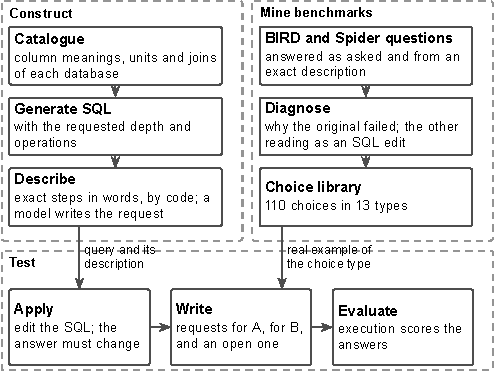
\includegraphics{diag_pipeline.pdf}
\caption{The \system{} pipeline.}
\Description{Two lanes of three boxes, Construct (catalogue, generate SQL, describe) and Mine (benchmark questions, diagnose,
decision library), both feed a bottom lane: apply a choice, write three requests, evaluate.}
\label{fig:pipeline}
\end{figure}
\subsection{Two examples}
\label{sec:worked}
\label{sec:test}
A request set fixes a database and every requirement of a query but one choice. The film request of Figure~\ref{fig:teaser} asks for each rating's average replacement cost and daily rental price, and compares that daily price with the average across ratings. Only the daily price is open:
\begin{equation}
 A=\operatorname{AVG}(\text{price}/\text{days}),\qquad
 B=\frac{\operatorname{AVG}(\text{price})}{\operatorname{AVG}(\text{days})}.
\end{equation}
A averages each film's daily price; B divides two averages and so gives more weight to longer rentals. The specific request for A asks for the average of per-film daily prices, the one for B asks for the average price divided by the average duration, and the open request asks for the ``average rental price per day.'' The rest of the wording is shared, and code checks that the two queries return different results on the database; a choice that does not change the answer is not tested there. \label{sec:additionalexample}The second example (Figure~\ref{fig:worked}) is a three-step query on the \texttt{insider} database. It averages short-interest measurements for each transaction, compares each transaction with a baseline for its order type, and returns the ten largest ratios. The choice lies in the baseline. Interpretation A averages the transaction means, so each transaction counts once, while B averages the underlying snapshots, so a transaction with more snapshots weighs more. The open request asks for ``the average short interest for its order type mix,'' and all ten output rows change between the interpretations.
% Built from figures/src/diag_worked.tex with pdfLaTeX (the paper's fonts); included at 1:1. Make in paper/tex rebuilds it.
% Values from out/paper/data/fig4_worked_example.json (case eval12@01cfbb1e713f-13e92662d1, database insider, arithmetic depth 1,
% step depth 3) and library/examples.jsonl (bird_pairs:b034).
\begin{figure}[t]
\centering
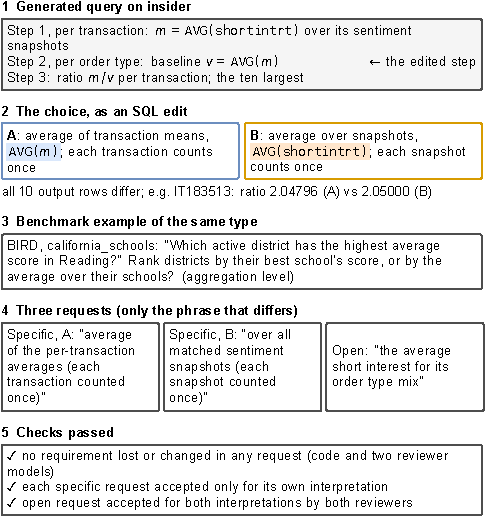
\includegraphics{diag_worked.pdf}
\caption{A request set on \texttt{insider}, from the generated query to its checks. Shaded: the SQL that differs.}
\Description{Five stacked boxes: the generated query with its edited step, the two interpretations and their executed difference, the
retrieved library example, the three requests, and the checks passed.}
\label{fig:worked}
\end{figure}

\subsection{Generating queries}
\label{sec:construction}
\label{sec:querygen}
\label{sec:writing}
Generation starts from the database, not from a benchmark, so it works on databases nobody has annotated. One model review of the schema and data first builds a catalogue of column meanings, units and table relationships; after that, generation calls no model. A query starts from counts, sums or averages per entity, per group or overall. Later steps can compare a value with a broader average, take a share of a total, combine compatible quantities, aggregate again, or keep the top entities per group. We control two properties of each query, its arithmetic depth (the nesting of arithmetic expressions) and its step depth (the number of dependent query stages). Rules on column types decide which quantities can be combined or summed, and data checks reject empty answers, constant or redundant quantities, non-positive denominators and too-small groups. The generator looks ahead and drops a partial query as soon as it can no longer reach the requested depths, so no attempt is spent on a dead end, and every delivered query has exactly the arithmetic and step depths it was asked for.

Code then describes each query exactly in words. The text covers source rows, joins, unmatched rows, filters, groups, formulas, missing values, ordering, limits, ties and SQLite conventions, and the same SQL always gives the same text; we call it the exact description. Because the exact description states every requirement, a model that fails from it cannot compute the query, while a model that succeeds from it but fails from a natural request was misled by the wording. Section~\ref{sec:library} builds on this contrast. Sonnet turns the exact description into one natural request using the column meanings. Claude Opus~5.5 (Opus below) checks the request for missing, changed or added requirements, and code checks how stored values are written. A failing request gets one revision with the reviewer's notes and is dropped if it fails again.

\begin{figure*}[t]
\centering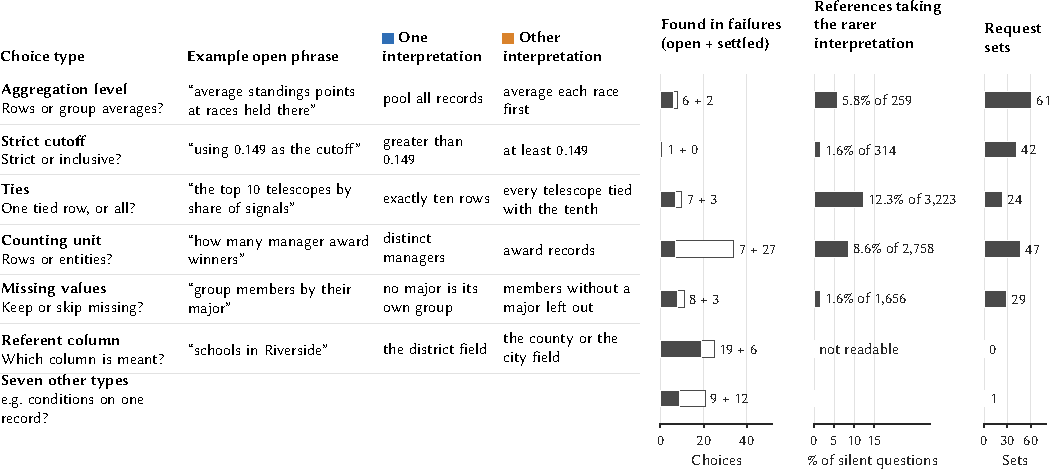
\includegraphics{col_choices.pdf}
\caption{Choice types: an example open phrase with its two interpretations, choices found in benchmark failures (gray: open; white: settled), silent BIRD and Spider references that take the rarer interpretation, and accepted request sets.}
\Description{One row per choice type with an example phrase, its two interpretations in blue and orange, and three bar panels: choices found in failures, references taking the rarer interpretation, and request sets.}
\label{fig:choices}
\end{figure*}

\subsection{Mining choices from benchmark failures}
\label{sec:library}
The choices come from real benchmark failures. For each BIRD and Spider question, we compare a model's answer to the original question (with BIRD's evidence) with its answer to the exact description of the reference SQL. When only the description is answered correctly, the wording caused the failure, not the model's SQL, and we classify the reason as output columns, a different column or value, an unstated requirement, numerical precision, or an open choice. For an open choice, the other interpretation is written as an edit of the reference SQL, and both queries are executed. Opus and Sonnet judge each interpretation independently, and disagreements are kept. The library keeps choices of meaning, both open ones, where the wording fits both interpretations, and settled ones, where it selects one. For ``What is the total number of molecules with double bonded oxygen?'', both reviewers accept only the interpretation in which the oxygen atom is part of the double bond, although the reference SQL counts every molecule that contains an oxygen atom and a double bond. Figure~\ref{fig:choices} groups the library by choice type. The largest group of open choices concerns which column a phrase refers to, and half of the settled ones concern the counting unit.

The same choices appear in benchmark references, and the references do not agree on them. We call a question silent on a choice when neither its wording nor BIRD's evidence contains a word that settles it, such as ``all'' for ties or ``distinct'' for counts. For 12 of the 13 choice types, code reads which interpretation a reference takes, and Figure~\ref{fig:choices} counts the silent BIRD and Spider questions and the share whose reference takes the rarer interpretation. Every case of the rarer interpretation was reviewed and only confirmed cases are counted, so these shares are conservative. For example, 12.3\% of silent tie questions return every tied row, and 8.6\% of silent counts over a join count distinct entities. Here a benchmark that scores one interpretation treats a convention as the only answer.



\subsection{Building request sets}
\label{sec:apply}
\label{sec:filters}
A request set needs a choice that matters on the data, so code first reports where a generated task's columns have missing values, repeated join matches, distinct values or ties. Opus proposes one choice from the library and an exact SQL edit for it, and code checks that the edit applies, runs, changes the answer and can still be described exactly; a failed proposal gets one repair. Opus then writes the request set from a plan that lists the shared requirements and the one differing choice. It writes the request for A, edits it for B, and writes the open request. A library example of the same type may guide the wording, but never supplies the SQL. Opus and Sonnet, as two reviewers, check that the requests keep their requirements and judge each of the three requests against each interpretation. A set is kept only when both reviewers accept each specific request for its own interpretation alone and at least one accepts the open request for both interpretations. Five library types concern a filter, such as whether a cutoff is strict. Generated queries seldom filter, so for these types the generator adds one condition chosen from the data. Figure~\ref{fig:choices} gives an example of each type. The pipeline keeps 307 request sets on 12 databases, and 204 of them pass the authors' review and a check against real references (Section~\ref{sec:specresults}).


% ===== metrics =====
\section{Measures}
\label{sec:metrics}
We score what a model computes by execution and what it says by a model judge. We report four measures: accuracy, both returned, named, and false alarms. A specific request selects one interpretation, and the open request fits both. A choice is settled when the wording selects one interpretation. We execute every returned query and compare its result with the reference result, with numerical tolerance and with rows tied at a cut-off treated as interchangeable; an execution error scores zero, as in Spider and BIRD scoring. For benchmark questions we also report a score that allows extra or reordered output columns.

For the open request, the model returns a main query and up to two alternatives. The model returns both interpretations when these queries include one with the result of A and one with the result of B. We report this share over all sets and over the sets in which the same model answers both specific requests correctly, where a miss cannot be a failure to compute. Written as a formula, with $S_i$ the queries returned for the open request of set $i$, $e(p,\hat p)=1$ when query $\hat p$ returns the result of reference $p$, and $B_i=1$ when both specific requests are answered correctly,
\begin{equation}
\mathrm{Both}=\frac{\sum_i B_i\prod_{j\in\{A,B\}}\max_{\hat p\in S_i}e(p_j,\hat p)}{\sum_i B_i}.
\end{equation} A missed interpretation is computable when the same model answers the specific request for it correctly. A model names the choice when its explanation says that the choice is open, whether or not it gives SQL for the other interpretation. A judge model, which does not know which model answered, decides whether a response names the choice and whether its stated interpretation matches its SQL. For a specific request, offering the other interpretation, or calling the choice open, is a false alarm. The measures check one another. Returning both interpretations alone would reward a model that adds every alternative it can think of, and the false alarms charge for that; naming alone would reward a warning without an answer, and returning both interpretations charges for the missing query. Table~\ref{tab:scoring} scores four recorded responses.

\begin{table}[t]
\caption{Four recorded responses and their scores.}
\label{tab:scoring}
\centering\footnotesize\setlength{\tabcolsep}{3pt}\renewcommand{\arraystretch}{1.15}
\providecommand{\cm}{\ensuremath{\checkmark}}\providecommand{\xm}{\ensuremath{\times}}
\begin{tabularx}{\columnwidth}{@{}>{\raggedright\arraybackslash}p{1.6cm}>{\raggedright\arraybackslash}p{1.45cm}Yccc@{}}
\toprule
Request, model & Main SQL & Alternative SQL & Names & Both & False alarm\\
\midrule
Film, open, GPT-Sol & A: mean of daily prices & none & \xm & \xm & \\
Film, open, GPT-Luna & A: mean of daily prices & none & \cm & \xm & \\
Awards, open, Sonnet & A: \sql{COUNT(*)} & B: \sql{COUNT(DISTINCT player\_id)} & \cm & \cm & \\
Fees, specific, Haiku & A, as asked & B: mean of channel means & & & \cm\\
\bottomrule
\end{tabularx}
\end{table}





On AMBROSIA, each ambiguous question comes with its interpretations, and an interpretation is found when some returned query gives its result. Recall is the share of interpretations found, and AllFound is the share of questions with every interpretation found~\cite{ambrosia2024}. Precision on an unambiguous question is the share of returned queries with its one correct result, so extras lower it.
% ===== evaluation =====
\section{Experimental Setup and Test Checks}
\label{sec:evaluation}
Sections~\ref{sec:disclosure}--\ref{sec:method} ask whether models report the choices they make, whether benchmarks see it, and how a system should report a choice and carry the user's pick. This section gives the setup (Section~\ref{sec:setup}) and checks that tests change only the choice (Section~\ref{sec:specresults}).

\subsection{Experiment settings}
\label{sec:setup}
\textbf{Data.} Request sets use 12 databases, four each from Spider, BIRD development and LiveSQLBench\footnote{\url{https://github.com/bird-bench/livesqlbench}}. The generated tasks request arithmetic depth 1--2 and step depth 3--6, and each database contributes 12 to 24 accepted request sets. Table~\ref{tab:data} lists the data.

\begin{table}[t]
\caption{The data and where each is used.}
\label{tab:data}
\centering\footnotesize\setlength{\tabcolsep}{3pt}
\begin{tabularx}{\columnwidth}{@{}>{\raggedright\arraybackslash}p{1.95cm}>{\raggedright\arraybackslash}X>{\raggedright\arraybackslash}p{1.05cm}@{}}
\toprule
Use & Data & Sections\\
\midrule
Request sets & 12 databases, four each from Spider (baseball, Sakila, customers-and-invoices, Chinook), BIRD (financial, student club, thrombosis prediction, Formula 1) and LiveSQLBench (archeology, insider, crypto, alien) & \ref{sec:apply}, \ref{sec:disclosure}, \ref{sec:method}\\
Mining choices & 481 BIRD development questions on five databases and 150 Spider development questions & \ref{sec:library}\\
Held-out test & 100 BIRD and 50 Spider development questions, never used for mining & \ref{sec:diagnosis}\\
Conventions & every BIRD and Spider question silent on a choice, training and development & \ref{sec:library}, \ref{sec:defaults}\\
Answer changes & every BIRD development question silent on a choice & \ref{sec:impact}\\
Method & AMBROSIA test split, ambiguous and unambiguous questions & \ref{sec:disclosure}, \ref{sec:method}\\
\bottomrule
\end{tabularx}
\end{table}

{\sloppy\textbf{Models.} We evaluate Haiku, Sonnet, GPT-Sol and GPT-Luna (\texttt{claude-haiku-4-5-20251001}, \texttt{claude-sonnet-5-5}, \texttt{gpt-6-sol}, \texttt{gpt-6-luna}). Opus writes the request sets, reviews them with Sonnet (Section~\ref{sec:apply}), reviews the natural requests that Sonnet writes for generated tasks (Section~\ref{sec:construction}), and judges the explanations; Opus is not evaluated. Models see the schema and documentation and have no file or tool access. By default a model answers in one call, with a prompt that asks for SQL, for a brief statement of ``any consequential assumption that the request and the supplied context do not settle,'' and for SQL of any other supported interpretation, without inventing alternatives. Computing is not our main question, so to test whether a model can compute an interpretation at all, we give it its best chance and let it explore. It may first run up to six rounds of five queries on the database, seeing twenty rows of each result. Exploration changes little: GPT-Sol solves 59 of 100 held-out BIRD questions without it and 61 with it, so one call is a fair default.\par}

\textbf{Statistics and baselines.} Intervals resample tasks 2,000 times, keeping pairs together; proportions use Wilson intervals; paired comparisons use exact McNemar tests. For our method (Section~\ref{sec:method}), we compare with the AMBROSIA authors' prompt, the same prompt sampled three times, disambiguate-then-parse (DtP)~\cite{saparina2025disambiguate}, and the products' interpret-and-state and ask-then-answer.



\subsection{Checks on the tests}
\label{sec:specresults}
\label{sec:resconstruction}
\label{sec:writerswap}
The findings rest on tests that change only the choice, so we check the tests first (Figure~\ref{fig:funnel}). Code confirms that in each of the 307 sets that pass all checks, the two queries differ in one step and the two specific requests differ only in the choice phrase. Two authors then cross-checked every set without seeing model results and kept it only if a reasonable analyst could mean either interpretation. They keep 232 of the 307 sets (76\%). Most rejected sets have an open request whose wording already favours one interpretation, or a choice that convention settles, such as ``between,'' which includes both ends in SQL and in almost every benchmark reference. We also keep only the choice types on which real references differ (Figure~\ref{fig:choices}), which leaves 204 sets on aggregation level, cutoffs, ties, counting units, missing values and one negation. Every result below uses these 204 sets. The review does not drive the results. With no human filter, models return both interpretations in only 11--48\% of the sets they can compute, so the gap holds without the review.

\begin{figure}[t]
\centering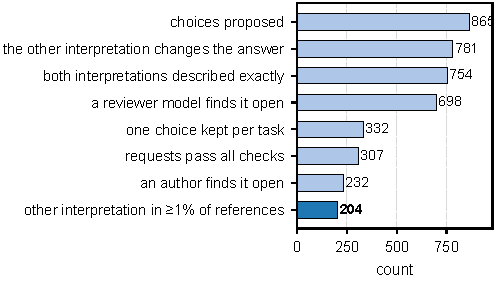
\includegraphics[width=\columnwidth]{col_funnel.pdf}
\caption{What each construction stage keeps, from proposed choices to accepted request sets.}
\Description{Horizontal bars decreasing from proposed choices to accepted request sets.}
\label{fig:funnel}
\end{figure}



The generator itself is reliable. Its rules find usable queries on 152 of the 190 Spider, BIRD and LiveSQLBench databases we tried; the others lack the repeated rows the rules need. On the 12 evaluation databases it delivers 1,198 of 1,200 requested queries, all at the requested depths, and each of its rules is needed (Figure~\extref{fig:ablation}); without the look-ahead, almost no attempt reaches its target. Natural requests also lose little against exact descriptions (Figure~\extref{fig:specification}). Sonnet and GPT-Sol lose about two points, and Haiku and GPT-Luna gain. Writing from a plan keeps the three requests aligned. On 60 tasks drawn at random across choice types, it keeps the shared requirements in 52 drafts, against 32 for direct generation ($p=0.0002$), and passes all checks in 49 against 32 drafts.

\textbf{No model favours its own family.} Claude models write and review the requests and Opus judges the explanations, so a Claude model might do better on them. We repeat each of these steps with GPT-Sol, from another family, and find no such advantage. When GPT-Sol writes the natural requests of 200 random generated tasks, neither GPT-Sol nor Sonnet gains on its own text. With exploration, GPT-Sol answers 395 of the 408 specific requests that Opus wrote, as many as Sonnet (396). When GPT-Sol rewrites the open requests of 60 random sets, no model returns both interpretations significantly more or less often (all $p\ge0.18$). The Opus judge does not favour Claude models either. It credits naming the choice in 96--100\% of responses that return both interpretations, and among responses that give one interpretation it credits GPT-Luna most often (27\%).









\section{Models Make Choices Without Saying So}
\label{sec:disclosure}
A model that computes both interpretations when each is asked for usually returns only one of them for the open request, and often does not say that there was a choice. Asking for an explanation does not cause this gap. Against the same call asking only for SQL, correct answers to specific requests change by at most nine of 204 per model, and every paired interval includes zero. Nor does it make models raise settled choices: at most two of 204 responses to specific requests per model call the choice open.

\begin{figure}[t]
\centering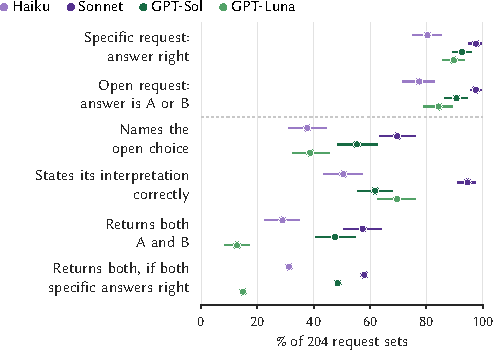
\includegraphics[width=\columnwidth]{col_disclosure.pdf}
\caption{Answering and communicating on 204 request sets, per model and measure (95\% intervals).}
\Description{Dot plot of five measures for four models with 95 percent intervals.}
\label{fig:disclosure}
\end{figure}

\textbf{Models return one interpretation where two are correct.} Returning both interpretations is much rarer than returning one correct answer (Figure~\ref{fig:disclosure}). Even among the sets in which a model answers both specific requests correctly, it returns both interpretations for the open request in only 58\% for Sonnet, 48\% for GPT-Sol, 31\% for Haiku and 15\% for GPT-Luna. Accuracy hardly separates the models, whose answers to specific requests are right in 80--98\% of sets, but reporting does. The larger model of each family returns both about two and three times as often as the smaller one, yet none closes the gap. When a model states its interpretation, the statement matches its SQL in 99--100\% of responses. The models describe one calculation correctly without saying that another, equally valid calculation was possible on the same data. The unreported interpretation matters. In 98 of the 204 sets, the two interpretations return different rows, and in the other 106 the same rows with different computed values, so the user gets a different answer in every set.

\textbf{Most misses are failures to report.} Most interpretations a model misses on the open request are ones it can compute. The same model computes the missed interpretation correctly when asked for it alone in 72--94\% of the missed sets (Figure~\ref{fig:decomposition}). Figure~\ref{fig:outcomes} sorts every open request into five outcomes, namely both interpretations returned, the choice named but one interpretation given, one interpretation given silently although the model computes both, a specific request computed wrong, and a specific answer whose SQL does not run. For Haiku and GPT-Luna the most common outcome is the silent one, in which the model can compute both interpretations but gives one without naming the choice, and for Sonnet and GPT-Sol it is the second most common. A score that only checks whether both interpretations appear among the outputs, as top-$k$ coverage~\cite{ambiqt2023} does, cannot tell these outcomes apart. Sampling does not surface the other interpretation either. On 55 randomly drawn sets, five SQL-only samples contain both interpretations in at most 14 for any model, while one explained response from Sonnet does so in 34. What is missing is a prompt to report the choice; SQL-only samples mostly repeat one interpretation.

\begin{figure}[t]
\centering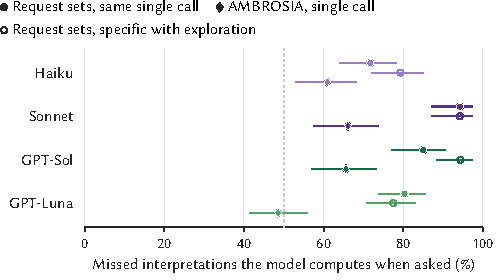
\includegraphics[width=\columnwidth]{col_decomposition.pdf}
\caption{Missed interpretations that the same model computes when asked for each of them alone, per model, on request sets with one call or after exploring the database, and on AMBROSIA (Wilson 95\% intervals).}
\Description{Dot plot with one row per model and three markers per row; most markers lie between 50 and 95 percent.}
\label{fig:decomposition}
\end{figure}

\begin{figure}[t]
\centering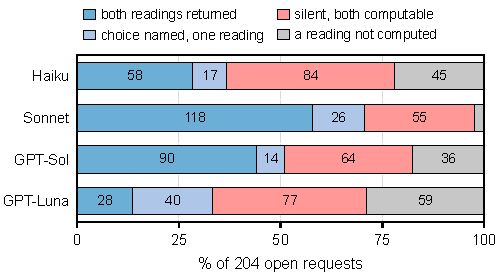
\includegraphics[width=\columnwidth]{col_outcomes.pdf}
\caption{What each model does with the 204 open requests (one call with explanation). Computable: the same call answers both specific requests correctly.}
\Description{Stacked horizontal bars, one per model, split into five outcomes; silent answers with both interpretations computable form the largest part for Haiku and GPT-Luna.}
\label{fig:outcomes}
\end{figure}

\textbf{The gap is widest for ties and counting units.} Sonnet, the best model, returns both interpretations for 68\% of aggregation-level sets but for only a third of tie and counting-unit sets, and the other models do worse (Figure~\ref{fig:bytype}). These choices hide in the SQL, in a \sql{LIMIT} or a \sql{COUNT} over a join, neither of which the request mentions. Cutoffs are the exception, because most cutoff requests give a value ``as the cutoff'' with no comparison word, which invites both the strict and the inclusive interpretation. The gap holds on every source of databases, and no model returns both interpretations for more than 67\% of the sets from any source.

\begin{figure}[t]
\centering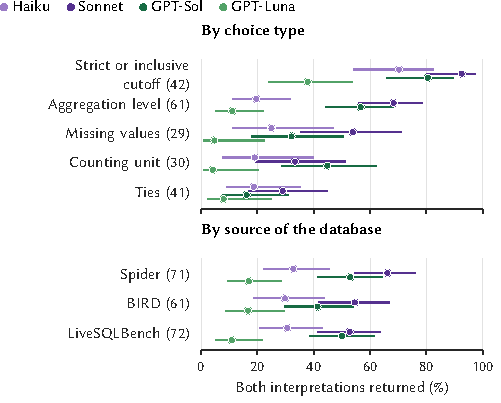
\includegraphics[width=\columnwidth]{col_bytype.pdf}
\caption{Open requests answered with both interpretations, by choice type and by source of the database, among the sets in which the same model answers both specific requests right (accepted sets in parentheses; Wilson 95\% intervals).}
\Description{Dot plot with five choice types and four models; cutoffs are high for three models, ties and counting units are low for all.}
\label{fig:bytype}
\end{figure}

\textbf{Naming a choice is not the same as giving the other interpretation.} A model that says a choice is open often stops there. Among the sets in which a model names the choice and can compute both interpretations in the same call, it still returns only one interpretation in 10--65\% of them, and GPT-Luna does so most often. Such a response warns the user but leaves them to write the other query, which is a step the model could have taken itself, since it computes that query when asked for it alone.

\begin{figure}[t]
\centering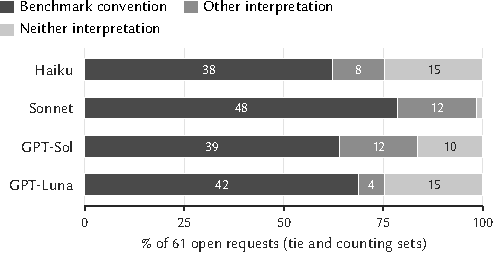
\includegraphics[width=\columnwidth]{col_conventions.pdf}
\caption{Main answer to the open request on 61 tie and counting sets: the interpretation BIRD and Spider references take by convention, the other interpretation, or neither.}
\Description{Stacked horizontal bars per model; the conventional interpretation outnumbers the other interpretation by at least three to one for every model.}
\label{fig:conventions}
\end{figure}

\textbf{Silent choices follow benchmark conventions.}\label{sec:filterresults} When a model settles a choice without saying so, it takes the interpretation that benchmark authors take. In 61 tie and counting sets, one interpretation is the convention of BIRD and Spider references (Section~\ref{sec:defaults}), namely a plain \sql{LIMIT} rather than every row tied at the cut-off, and counting joined rows rather than distinct entities. The conventional interpretation is the intended one in 29 of these sets, so the design favours neither. Yet when a model's main answer is one of the two interpretations, it is the conventional one in 76--91\% of cases for every model (Figure~\ref{fig:conventions}). The conventional interpretation is also the simpler SQL, so these data cannot separate habit from simplicity. Either way, models settle an open choice the way benchmark authors do, which is also the interpretation that a benchmark built by those authors rewards.

\textbf{The same holds on AMBROSIA.} The pattern is not an artifact of our tests. AMBROSIA pairs each ambiguous question with one unambiguous question per interpretation, and Saparina and Lapata~\cite{saparina2025disambiguate} observe that models usually give one preferred interpretation. We split each missed interpretation into one the model cannot compute and one it computes but does not report. On 120 ambiguous test questions per model, the model computes 49--66\% of the interpretations it misses when asked the unambiguous version (Figure~\ref{fig:decomposition}). Even when a model answers every unambiguous version correctly, it returns all interpretations for the ambiguous question in only 12--28\% of questions. On the 40 vagueness questions per model, which ask which column or value a phrase means, models compute 48--56\% of the interpretations they miss, so the gap also covers the referent-column choices that our request sets leave out. On both benchmarks, models compute what is asked and stay quiet about settled choices, but leave open choices unreported, whatever the source of the ambiguity, wording or calculation.

\textbf{Examples.}\label{sec:examples} For the film request of Figure~\ref{fig:teaser}, GPT-Sol states interpretation A, which matches its SQL, but treats the choice as settled; GPT-Luna says the choice is open but gives no second query; Sonnet adds B: ``per-day price defined as the rating's average rental\_rate divided by its average rental\_duration (ratio of averages).'' Responses can also mislead in the other direction. For a specific request on fees, Haiku computes a mean of channel means, which matches the other interpretation and contradicts the request; for an open count of awards, Sonnet names the choice and gives both \sql{COUNT(*)} and \sql{COUNT(DISTINCT player\_id)}, the two counting units.




\section{Benchmarks Cannot See the Gap}
\label{sec:diagnosis}
BIRD and Spider score a model against one interpretation even where a question leaves the choice open, and which interpretation they take depends on who wrote the question. On held-out questions, the four models answer 49--74\% of BIRD questions correctly as worded but 96--100\% from the exact description of the reference SQL (Figure~\ref{fig:real}). Allowing extra or reordered output columns closes only part of this gap, and on Spider the remaining gap is smaller.

\begin{figure}[t]
\centering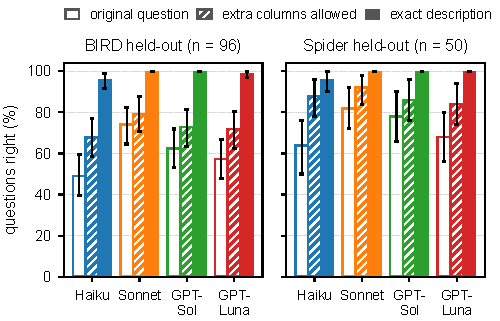
\includegraphics[width=\columnwidth]{col_real.pdf}
\caption{Held-out questions: original question versus the exact description of the reference SQL (95\% intervals).}
\Description{Grouped bars for four models on BIRD and Spider held-out questions under three conditions.}
\label{fig:real}
\end{figure}

The exact description gives the reference's steps, columns and choices at once, so this gap bounds what the wording costs rather than measuring ambiguity alone. To see what it consists of, Opus assigns one cause to each development question answered correctly from the description and wrongly as worded (Figure~\ref{fig:causes}). Output columns, a phrase mapped to another column or value, unstated requirements and run-to-run variation cause most failures. A second labeler from another family, GPT-Sol, given the same evidence, agrees on the cause for 53\% of the questions (Cohen's $\kappa=0.44$); it often calls Opus's run-to-run variation output shape and finds an open choice in 35 questions where Opus finds 16, so the figure, if anything, undercounts open choices. Output columns are a matter of form, as the answer holds the right values in a different shape, such as a name instead of an ID. Open choices, which our library collects, are one of these causes. Failures undercount them, because an answer following the benchmark's convention is scored right; Section~\ref{sec:impact} measures them on every silent question.

Other choices are about which column a word means. For ``Name schools in Riverside\ldots'', filtering the district field returns six rows, the county field sixty and the city field seven. Code cannot tell from a reference which column the question's word could also mean, so request sets leave this type to AMBROSIA's vagueness questions.






\begin{figure}[t]
\centering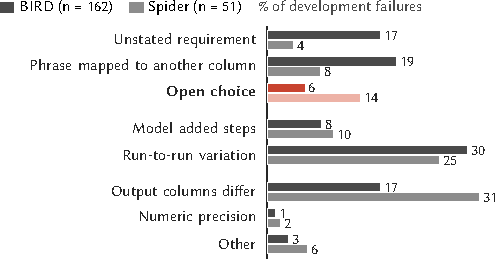
\includegraphics[width=\columnwidth]{col_causes.pdf}
\caption{Why the original question failed, on development questions answered right from the exact description and wrong as worded, one cause per question.}
\Description{Eight causes, one row each, with a bar for BIRD and one for Spider; open choices are shown in red.}
\label{fig:causes}
\end{figure}



\subsection{References follow unstated conventions}
\label{sec:defaults}
When a question is silent on a choice, its reference still takes one interpretation, and the interpretation depends on the author group. We read seven such choices off reference SQL, among them ties at an extreme, counting over a join, join type, and whether ``between'' includes its bounds. On five of the seven, every author group takes the same interpretation in at least 91\% of silent questions. On ties and counting, the groups disagree (Figure~\ref{fig:defaults}). Asked for an extreme value, BIRD and Spider references return one row in over 90\% of silent questions, but the Geo and Restaurants questions that Spider imported from older datasets return one row in 21 of 247. Asked for a count over a join, BIRD references count joined rows in most silent questions, and the imported Academic, IMDB and Yelp questions in none of 39. Each group keeps its convention in training and development data alike, so examples retrieved from a benchmark's training data can carry its authors' convention into a model's answers. For the same wording, a model that follows BIRD's convention is therefore scored right on BIRD and wrong on the imported Spider questions. The score measures agreement with the benchmark authors, not correctness.

\begin{figure}[t]
\centering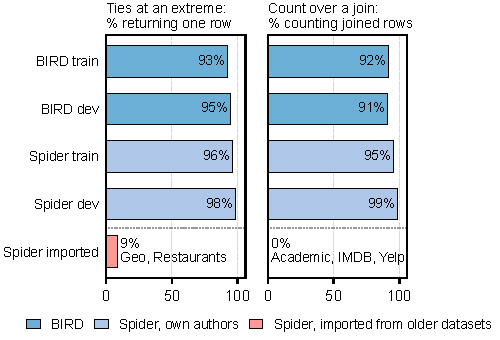
\includegraphics[width=\columnwidth]{col_defaults.pdf}
\caption{Share of silent questions whose reference takes the usual interpretation, by author group, for the two choices on which groups disagree, ties and counting.}
\Description{Two panels of horizontal bars. BIRD and Spider bars are at 91 to 99 percent; the imported Spider groups are at 9 percent (ties) and 0 percent (counting).}
\label{fig:defaults}
\end{figure}

\begin{table}[t]
\caption{Six of the 17 BIRD questions on which all four models return the other interpretation, confirmed by two of us; BIRD scores each of these answers wrong.}
\label{tab:answers}
\centering\footnotesize\setlength{\tabcolsep}{3pt}\renewcommand{\arraystretch}{1.15}
\begin{tabularx}{\columnwidth}{@{}Y>{\raggedright\arraybackslash}p{1.75cm}>{\raggedright\arraybackslash}p{1.75cm}@{}}
\toprule
Question & BIRD reference & Other interpretation\\
\midrule
``Who is the tallest superhero?'' & 1 hero & 2 tied heroes\\
``\ldots\ cards in the set Coldsnap with the highest converted mana cost.'' & 1 card & 12 tied cards\\
``What are the expenses of the budget with the lowest remaining?'' & 1 expense & 2 tied expenses\\
``How many of the banned cards are white border?'' & 258 rows & 89 cards\\
``\ldots\ normal glutamic pylvic transaminase level, how many of them are male?'' & 1{,}924 lab records & 45 patients\\
``\ldots\ diagnosed with SJS, how many of them have a normal level of total protein?'' & 780 lab records & 37 patients\\
\bottomrule
\end{tabularx}
\end{table}

\subsection{The unstated interpretation changes answers}
\label{sec:impact}
The choice a reference makes silently is not cosmetic. For each BIRD development question that is silent on a choice, we apply the library's edit for the other interpretation to the reference SQL wherever it gives a valid interpretation, and run both. Of 664 such questions, 156 (23\%) change their answer (Figure~\ref{fig:impact}). These are one in ten of all BIRD development questions. Counting moves the answer most, often by more than half of its value. For ``How many accounts in North Bohemia has made a transaction with the partner's bank being AB?'', the reference counts joined rows and returns 2,260, while counting each account once returns 55. Ties change about a quarter of answers, often the list of returned items, and join type and missing-value filters change about one in ten. The data behind these choices are common. Every one of the 12 evaluation databases has at least two kinds of data on which an unstated choice changes an answer, such as joins that repeat rows, columns with missing values and maxima shared by several rows.

\textbf{BIRD scores the other interpretation as wrong.} On the 79 questions checked below, accepting both interpretations raises accuracy from 25\% to 57\%; the difference is answers that BIRD counts as wrong SQL, although the question allows them. We ask the four models 137 BIRD development questions on which a tie, counting or join edit of the reference changes the answer, and score each answer against both queries. Two authors checked that the edit gives a valid interpretation of the question, and 79 questions pass. Of the 236 answers BIRD marks wrong on them, 99 return the other interpretation. On tie and counting questions, more answers match the edited reference (90) than the reference itself (37), and on 17 questions every model returns the other interpretation (Table~\ref{tab:answers}).

\begin{figure}[t]
\centering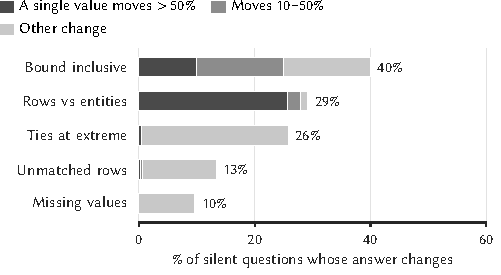
\includegraphics[width=\columnwidth]{col_impact.pdf}
\caption{Silent BIRD development questions whose answer changes under the other interpretation, by choice type and by how far a single answer value moves.}
\Description{Stacked horizontal bars for five choice types; inclusive bounds change 40 percent of answers and counting rows versus entities 29 percent, mostly with values moving by more than half.}
\label{fig:impact}
\end{figure}
% ===== method =====
\section{A Two-Phase Method for Open Choices}
\label{sec:method}
A conversation about an open choice has two moments, before the user says which interpretation they mean and after. Production assistants ask or return one interpretation before (Section~\ref{sec:intro}) and rewrite the request after (Section~\ref{sec:rewrite}). Our method has one phase for each moment, and each step follows from a finding of this paper. Models state their interpretation accurately and almost never call a settled choice open (Section~\ref{sec:disclosure}), so one call can decide whether a choice is open; they compute most interpretations they miss once each is asked for alone, so each gets its own call; and a rewrite keeps the choice but loses other requirements (Section~\ref{sec:rewrite}), so each interpretation is written as the full request and the pick is added as one clause, leaving the rest word for word.

\subsection{Phase 1: decide, then answer}
\label{sec:methoddesign}
Phase 1, decide-then-answer, runs before the user replies (Figure~\ref{fig:methodsteps}). First, one call lists the interpretations of the request, each written as the full request with exactly one interpretation; if it lists only one, one more call answers it, and nothing else runs, so a clear request costs two calls and one query. Second, where a choice is open, each interpretation it lists, at most four, is answered in its own call. Third, every answer runs on the database, SQL that fails is dropped, and identical results are shown once. The user sees the first answer with the others as alternatives, and phase 2 starts when the user picks one (Section~\ref{sec:rewrite}). An option, decide-then-search, first searches wide in the second step, with two more calls that list the interpretations and then any that are missing, using DtP's prompts~\cite{saparina2025disambiguate}.

% Built from figures/src/diag_method.tex with pdfLaTeX; the two results are the real sakila_1 values of Figure 1.
\begin{figure}[t]
\centering
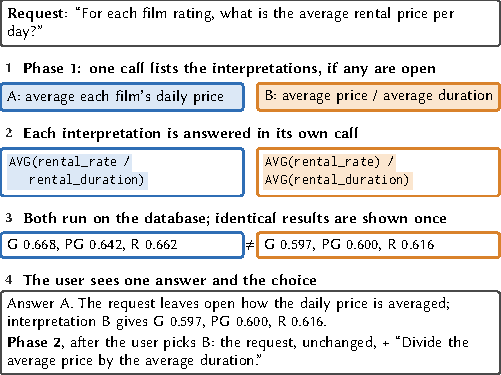
\includegraphics{diag_method.pdf}
\caption{Both phases on the film request. Blue and orange: interpretations A and B, as in Figure~\ref{fig:teaser}.}
\Description{Four steps: decide whether a choice is open and list the interpretations, answer each in its own call, run both and compare the results, show one answer with the choice and carry the user's pick as one added clause.}
\label{fig:methodsteps}
\end{figure}

\subsection{Phase 1 against products and baselines}
\label{sec:methodambrosia}
\label{sec:exchange}
We developed the method on 60 AMBROSIA questions. The final test uses 150 new test questions per model (90 ambiguous, 60 unambiguous) and 111 randomly drawn request sets, with Sonnet and GPT-Sol. We compare it and its option with the AMBROSIA authors' prompt (plain), the same prompt sampled three times, DtP with its released prompts, and interpret-and-state, the single answer that production assistants return in the same turn with their interpretation, like Cortex Analyst's ``We interpreted your question as\ldots''~\cite{cortexdocs2025}; execution scores its answer, the plain call's main query.

\begin{figure}[t]
\centering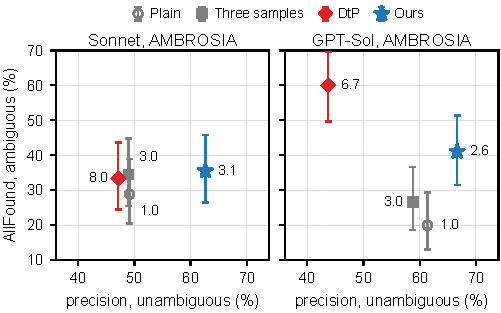
\includegraphics[width=\columnwidth]{col_method.pdf}
\caption{Methods on 150 new AMBROSIA test questions per model; calls per question beside each point (95\% intervals).}
\Description{Two scatter panels, Sonnet and GPT-Sol: decide-then-search, decide-then-answer, plain, three samples, DtP and interpret-and-state.}
\label{fig:method}
\end{figure}

% >>> table methods (generated by specbridge.report.tables_tex; do not edit by hand)
\begin{table}[t]
\caption{Decide-then-answer, decide-then-search and four baselines, among them interpret-and-state, the single answer that production assistants return, measured the same way on both datasets: coverage (all interpretations returned, of 90 ambiguous AMBROSIA questions and 111 open requests), precision on clear or specific requests (\%), and calls per request. Bold: best per model.}
\label{tab:methods}
\centering\footnotesize\setlength{\tabcolsep}{3.2pt}
\begin{tabular}{@{}llrrrrrr@{}}
\toprule
& & \multicolumn{3}{c}{AMBROSIA} & \multicolumn{3}{c}{Request sets} \\
\cmidrule(lr){3-5}\cmidrule(l){6-8}
Model & Method & Cover & Prec. & Calls & Cover & Prec. & Calls \\
\midrule
Sonnet & Plain & 26 & 49.1 & \textbf{1.0} & 64 & 94.6 & \textbf{1.0} \\
 & Three samples & 31 & 49.0 & 3.0 & 72 & 92.0 & 3.0 \\
 & DtP & 30 & 47.1 & 8.0 & 10 & 18.6 & 8.0 \\
 & Interpret-and-state & 9 & \textbf{65.0} & \textbf{1.0} & 0 & \textbf{98.2} & \textbf{1.0} \\
 & Decide-then-answer & 32 & 62.6 & 3.1 & 78 & 96.1 & 2.6 \\
 & \quad decide-then-search & \textbf{37} & 54.0 & 8.7 & \textbf{79} & 89.2 & 6.7 \\
\midrule
GPT-Sol & Plain & 18 & 61.4 & \textbf{1.0} & 47 & 83.3 & \textbf{1.0} \\
 & Three samples & 24 & 58.8 & 3.0 & 60 & 82.6 & 3.0 \\
 & DtP & \textbf{54} & 43.7 & 6.7 & 35 & 67.3 & 5.3 \\
 & Interpret-and-state & 8 & 65.0 & \textbf{1.0} & 0 & 82.9 & \textbf{1.0} \\
 & Decide-then-answer & 37 & \textbf{66.7} & 2.6 & 62 & \textbf{93.7} & 2.5 \\
 & \quad decide-then-search & 45 & 65.4 & 6.0 & \textbf{68} & 91.5 & 5.3 \\
\bottomrule
\end{tabular}
\end{table}
% <<< table methods

\textbf{More interpretations than today's answer, at no loss of precision.} Table~\ref{tab:methods} measures both datasets the same way: coverage, the open requests with every interpretation returned; precision, the share of returned answers that are right on clear or specific requests; and calls. Pooled over both models and paired by item, decide-then-answer returns every interpretation for 28.9 points more ambiguous AMBROSIA questions than interpret-and-state ($[22.2, 35.6]$) and for 63.1 points more open requests ($[57.2, 69.4]$), with no loss of precision ($-0.3$ points on AMBROSIA, $[-7.7, 7.2]$; $+4.4$ on request sets, $[0.5, 8.4]$), and its main answer is right on 6.3 points more specific requests. Against plain prompting, three samples and DtP, it is the most precise, by 9.4 to 19.2 points on AMBROSIA and 5.9 to 52.0 points on request sets, all significant; it covers more than plain prompting and three samples, and more than DtP on request sets, where DtP's restatements lose other requirements (42.8 points). Only on AMBROSIA does DtP cover more, by 8.3 points, at 19.2 points less precision and nearly three times the calls.

\textbf{Where the gain comes from.} Decide-then-search is DtP with the first step added, so their difference isolates that step: the same AllFound ($-1.1$ points) and 14.3 points more precision. The gain is not from returning fewer alternatives. We cut DtP's answers, per question, to the number of interpretations that the first step lists. Spent where the first step finds a choice, this budget finds every interpretation on 7.6 points more ambiguous questions than spent on random questions ($[3.8, 11.3]$), and decide-then-answer, with the same budget, finds 15.0 points more than the cut DtP ($[9.4, 20.6]$) at no lower precision. Decide-then-search finds every interpretation for 7.2 points more ambiguous questions but is 5.0 points less precise, at 2.3 times the calls, so it suits users who must miss no interpretation, whatever the calls cost.

\textbf{Fewer turns than asking the user.} Products also settle an open choice over two turns: Genie asks a clarifying question~\cite{genie2025}, and a Cortex Analyst user can correct the stated interpretation. A simulated user with one interpretation in mind states it in one more turn when no shown answer gives it, and the model then answers the specific request, the same second answer for every method. Ask-then-answer asks wherever our first call finds a choice open, which favours asking. Per 100 requests, with one in five AMBROSIA questions ambiguous, decide-then-answer needs 35.0 fewer user turns than ask-then-answer ($[28.8, 42.1]$) and 14.9 fewer than interpret-and-state ($[9.6, 20.6]$), and 40.8 and 22.1 fewer on request sets. It also ends right on 9.1 and 12.6 more AMBROSIA requests and on 3.4 and 6.1 more request-set requests, all significant, because an answer shown in the first turn needs no second answer that can go wrong, at 1.1 to 1.5 more calls per request.

\subsection{Phase 2: keep the request, add the pick}
\label{sec:rewrite}
When the user picks an interpretation, today's systems rewrite the request. Cortex Analyst rewrites each follow-up into a self-contained question~\cite{xu2024cortex}, the Fabric data agent rephrases each question~\cite{fabric2026agent}, LangChain's ConversationalRetrievalChain~\cite{langchain2024crc} and LlamaIndex's CondenseQuestionChatEngine~\cite{llamaindex2024condense} condense each follow-up into a standalone question, and DtP writes each interpretation as a short question. Each rewrite is a new copy that can lose a requirement, so phase 2 keeps the request and adds the pick as one clause, leaving the rest unchanged.




Request sets test this, as their three requests differ only in the choice. For each interpretation of a request set, the same SQL prompt receives one of four texts: (a) the original specific request; (b) the open request rewritten by the model as one interpretation with DtP's prompt, told the intended interpretation; (c) the open request unchanged, followed by a one-sentence description of the interpretation; (d) the open request and the interpretation condensed by the model into a standalone question with LangChain's prompt~\cite{langchain2024crc}; we report 363 interpretations drawn at random from the 204 sets, with all four models and one SQL prompt.

\begin{figure}[t]
\centering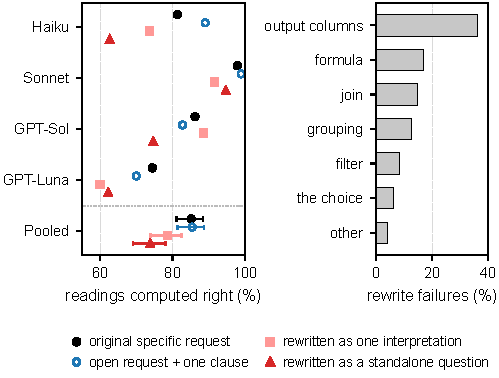
\includegraphics[width=\columnwidth]{col_rewrite.pdf}
\caption{Editing versus rewriting a request (363 interpretations). Left: interpretations computed right from four request texts. Right: what the rewrite lost, by kind.}
\Description{Left: dot plot per model of accuracy for four request texts; the two rewrites lie below the edited request. Right: horizontal bars, formula largest.}
\label{fig:rewrite}
\end{figure}

Keeping the request and adding one clause computes 80.7\% of the interpretations correctly, as many as the original specific requests ($p=0.57$, exact McNemar; Figure~\ref{fig:rewrite}). Both rewrites compute fewer, 8.5 points fewer for the interpretation rewrite ($p=0.0004$) and 10.5 for the standalone question ($p<0.0001$), and the loss is largest for Haiku and GPT-Luna. The rewrite seldom loses the choice itself. Of the interpretations answered correctly from the original request and wrongly from the rewrite, the judge finds the choice lost in only 12\%; the rest lose another requirement, most often a formula, an output column or a join (Figure~\ref{fig:rewrite}, right).



\textbf{The same holds on real questions.} We repeat the comparison on 85 BIRD development questions where one library edit of the reference SQL changes the answer. A simulated user follows each question with one sentence that settles the choice, such as ``If several rows tie at the cut-off, return all of them,'' and the edited reference is the gold answer. Over 170 question--model pairs with Sonnet and GPT-Sol, adding the clause beats the standalone question, 58.2\% against 47.6\%. As on our request sets, the rewrite keeps the clarified choice and loses something else; the gap is largest for ties.
% ===== discussion =====
\section{Implications}
\label{sec:lessons}
\textbf{Systems could answer open choices instead of asking.} A model states its interpretation accurately and can usually compute the other one, yet seldom reports it. Deciding first, answering each interpretation on its own and executing the answers already adds the other interpretations to an assistant's answer at no loss of precision and saves the user turns that asking costs (Section~\ref{sec:method}).

\textbf{Reporting could be a training target.} The models we test already compute both interpretations of most requests; what they mostly lack is the habit of reporting the second one. Sonnet, the strongest model, still misses it in four of ten sets where it can compute it, so training may help more than scale, and request sets could supply the signal. Each interpretation has its own executable reference, so a reward can credit an open answer only when it returns both interpretations and charge a specific answer for every alternative it adds, which rewards reporting but not guessing.

\textbf{Benchmarks could reward stating assumptions.} Current benchmarks score a single answer per question, which suits questions with one correct interpretation. For a question that is silent on a choice, a complementary practice is to let the model state the assumption it made and the alternative it set aside, and to credit both when each matches its own reference. Request sets make this possible because each interpretation has its own reference, so a benchmark can report accuracy on specific requests, reporting on open requests, and restraint on settled ones.

\section{Related Work}
\label{sec:related}
\textbf{Natural language interfaces to databases.} NaLIR~\cite{nalir2014} fixed ``easy'' ambiguities quietly and, for each ``hard'' one, explained its interpretation and offered several for the user to choose from. Its ambiguities lie mainly in mapping words to schema elements and in how phrases attach. Our results show that the alternatives NaLIR asked users to choose among are now cheap to compute; what is missing is the report. Our method applies NaLIR's interaction to calculation choices and lets execution decide which are ``hard''.

\textbf{Evaluation.} Spider tests generalization across schemas~\cite{spider2018}; BIRD adds large databases and external knowledge~\cite{bird2023}; KaggleDBQA uses realistic databases and documentation~\cite{kaggledbqa2021}; Spider 2.0 tests enterprise workflows~\cite{spider22025}. SParC and CoSQL add context and dialogue~\cite{sparc2019,cosql2019}, and BIRD-INTERACT tests clarification and recovery~\cite{birdinteract2026}. It scores whether a system completes a task after asking the user, whereas request sets score whether it reports a choice it made without asking. TrustSQL rewards a model for abstaining when it cannot answer reliably and penalizes wrong answers~\cite{lee2024trustsql}; request sets reward a different behaviour, answering while reporting the open choice. Error detectors flag executable SQL that is wrong against one gold query~\cite{chen2023error}, and verifiers turn such silent failures into abstentions~\cite{alrashed2026verification}; a silent choice passes both, because its SQL is correct for one interpretation. Test suites~\cite{testsuite2020} catch wrong queries whose results match by chance; our concern is the opposite error, in which a correct query for another valid interpretation is rejected because the reference fixes one interpretation. Pourreza and Rafiei re-evaluated top models on Spider and BIRD by hand and found a perfect score out of reach ``due to the multiple interpretations that can be derived from the provided samples''~\cite{pourreza2023evaluating}, and Wretblad et al.\ found noise in BIRD's questions and references whose correction changed which method ranks first~\cite{wretblad2024noise}. We measure the first problem by construction rather than inspection and keep possible reference errors apart from open choices, because a wrong reference and a valid but different one need different fixes.

\textbf{Ambiguous requests.} The closest benchmarks are AmbiQT~\cite{ambiqt2023} and AMBROSIA~\cite{ambrosia2024} (Table~\ref{tab:comparison}). AmbiQT makes Spider questions ambiguous by changing the schema, with synonym columns or tables, split tables and precomputed aggregates, and checks whether both gold queries appear in the top five outputs. AMBROSIA has human-written questions with scope, attachment and vagueness ambiguity on generated databases. Both locate ambiguity in the schema or the wording. The choices behind the conventions of Section~\ref{sec:defaults}, such as ties, counting units, missing values and aggregation level, lie in the calculation, outside both taxonomies. Outside SQL, AmbigQA asks for every plausible answer to an ambiguous question~\cite{min2020ambigqa}, and conversational search studies when a system should ask a clarifying question~\cite{aliannejadi2019asking}. In text-to-SQL the choice often lies in the calculation, where a model can answer fluently without noticing it, so request sets test reporting apart from computing.

\textbf{Generation, SQL methods and semantic layers.} DBPal~\cite{dbpal2020} and GAZP~\cite{gazp2020} generate training pairs for a target database; We also start from the database, but for evaluation. RAT-SQL, PICARD, DIN-SQL, DAIL-SQL, CHASE-SQL and Alpha-SQL~\cite{ratsql2020,picard2021,dinsql2023,dailsql2024,chasesql2025,alphasql2025} improve how the SQL is generated. Methods that retrieve training examples, such as DAIL-SQL, can carry the benchmark authors' conventions into the answers, so part of a benchmark gain may come from matching them. LookML has developers write each measure ``once, in one place''~\cite{lookml2025}, the dbt Semantic Layer centralizes metric definitions~\cite{dbtsl2025}, and Cortex Analyst generates SQL from them~\cite{cortexdocs2025}. A layer settles the choices its authors foresaw, usually a measure's formula and counting unit; per-request choices, such as ties or the rows a ratio includes, stay open, and these are the choices our method finds and answers for the user.

\section{Conclusion}
\label{sec:discussion}
Text-to-SQL models make choices without saying so. Request sets, which change only one calculation choice, make this visible. Four models compute both interpretations of most sets when each is asked for, yet return both for the open request in only 15--58\% of those sets, and when they settle a choice silently, they take the interpretation that benchmark references take by convention. Benchmarks cannot see the gap, because their references take one interpretation by conventions that differ by author group; over two in five answers BIRD marks wrong on such questions give the other interpretation. A method that decides first whether a choice is open and answers each interpretation on its own misses fewer interpretations than plain prompting, shows far fewer wrong answers than sampling and DtP, adds what production assistants' single answer drops at no loss of precision, needs fewer user turns than asking, and keeps the request when the user picks. The models already hold the other interpretation; what is missing is a step that shows it to the user, and a benchmark that asks for it and rewards it. Until then, a plausible number from a text-to-SQL system can answer a different question than the analyst asked, and nothing in the answer says so. We release the request sets, the library of choices, every model response and the code that scores them.

\textbf{Limitations and future work.} The generator covers a subset of analytical SQL, and the library comes from two benchmarks on SQLite, so other benchmarks may hold choice types we have not seen. The request sets cover every choice type on which real references differ, except quantifier, which the generator does not yet build, and referent column, which code cannot read off a reference; for the latter, AMBROSIA's vagueness questions show the same gap. Each request set tests one choice at a time, so requests that leave two choices open at once are not covered. The conventions are read by rules that see one SQL form each, so their counts are lower bounds. One model family wrote the request sets, but the results hold with another writer and without the human review (Section~\ref{sec:specresults}). The BIRD rescoring uses one call per question without exploration, so its shares may shift with stronger prompting. Interpret-and-state and ask-then-answer are rebuilt from the products' documentation, not run on the products, and the two-turn test uses a simulated user, not real users. A model judge decides whether a response names the choice, but execution decides every accuracy score and whether both interpretations are returned. Other SQL dialects and a study of how real analysts act on a reported choice come next.
\clearpage % the body fills pages 1-12; references start on page 13
\bibliographystyle{ACM-Reference-Format}
\bibliography{references}
\end{document}
